\subsection{Projective likelihood estimator (PDE approach)}
\label{sec:likelihood}

The method of maximum likelihood\index{Likelihood} consists of building a 
model out of probability density functions (PDF)\index{PDF}\index{Probability Density Function} that reproduces the input 
variables for signal and background. For a given event, the likelihood for 
being of signal type is obtained by multiplying the signal probability densities 
of all input variables, which are assumed to be independent, and normalising this 
by the sum of the signal and background likelihoods. Because correlations among 
the variables are ignored, this PDE approach is also called ``naive Bayes estimator'', 
unlike the full multidimensional PDE approaches such as PDE-range search, 
PDE-foam and k-nearest-neighbour discussed in the subsequent sections, which 
approximate the true Bayes limit. 

\subsubsection{Booking options}

The likelihood classifier is booked via the command:
\begin{codeexample}
\begin{tmvacode}
factory->BookMethod( Types::kLikelihood, "Likelihood", "<options>" );
\end{tmvacode}
\caption[.]{\codeexampleCaptionSize Booking of the (projective) likelihood classifier: 
         the first argument is the predefined enumerator, the 
         second argument is a user-defined string identifier, and the third argument 
         is the configuration options string. Individual options are separated by a ':'. 
         See Sec.~\ref{sec:usingtmva:booking} for more information on the booking.}
\end{codeexample}

The likelihood configuration options are given in Option 
Table~\ref{opt:mva::likelihood}.

% ======= input option table ==========================================
\begin{option}[!t]
\input optiontables/MVA__Likelihood.tex
\caption[.]{\optionCaptionSize 
     Configuration options reference for MVA method: {\em Likelihood}.
     Values given are defaults. If predefined categories exist, the default category 
     is marked by a '$\star$'. The options in Option Table~\ref{opt:mva::methodbase} on 
     page~\pageref{opt:mva::methodbase} can also be configured.
     
}
\label{opt:mva::likelihood}
\end{option}
% =====================================================================

\subsubsection{Description and implementation}
\label{sec:likelihood:description}

The likelihood\index{Likelihood} ratio $\RLik(i)$ for event $i$ is defined by
\beq
\label{eq:RLik}
	\RLik(i) = \frac{\Lik_S(i)}{\Lik_S(i) + \Lik_B(i)}\,,
\eeq
where 
\beq
\label{eq:Likelihood}
	\Lik_{S(B)}(i) = \prod_{k=1}^\Nvar p_{S(B),k}(x_k(i))\,,
\eeq
and where $p_{S(B),k}$ is the signal (background) PDF for the $k$th
input variable $x_k$. The PDFs are normalised 
\beq
\label{eq:pdfNorm}
	\intl_{-\infty}^{+\infty}p_{S(B),k}(x_k) dx_k = 1\,, \hspace{0.5cm}\forall k.
\eeq
It can be shown that in absence of model inaccuracies (such as correlations
between input variables not removed by the de-correlation procedure, or an inaccurate
probability density model), the ratio~(\ref{eq:RLik}) provides optimal signal from 
background separation for the given set of input variables. 

Since the parametric form of the PDFs is generally unknown, the PDF shapes are empirically
approximated from the training data by nonparametric functions, which can be 
chosen individually for each variable and are either  polynomial 
splines of various degrees fitted to histograms or unbinned kernel density estimators (KDE),
as discussed in Sec.~(\ref{sec:PDF}). 

A certain number of primary validations are performed during the PDF
creation, the results of which are printed to standard output.
Among these are the computation
of a $\chi^2$ estimator between all nonzero bins of the original 
histogram and its PDF, and a comparison of the number of outliers 
(in sigmas) found in the original histogram with respect to the 
(smoothed) PDF shape, with the statistically expected one. The 
fidelity of the PDF estimate can be also inspected visually by executing 
the macro \code{likelihoodrefs.C} (\cf\  Table~\ref{pgr:scripttable2}).

\subsubsection*{Transforming the likelihood output\index{Likelihood output transformation}}

If a data-mining problem offers a large number of input variables, or 
variables with excellent separation power, the likelihood response $\RLik$ 
is often strongly peaked at 0 (background) and 1 (signal). Such a response
is inconvenient for the use in subsequent analysis steps. TMVA therefore 
allows to transform the likelihood output by an inverse sigmoid function
that zooms into the peaks
\beq
\label{eq:RLikTransformed}
		\RLik(i) \longrightarrow \RLik^\prime(i) = 
		-\tau^{-1}\ln\!\left(\RLik^{-1}-1\right)\,,
\eeq
where $\tau=15$ is used. Note that $\RLik^\prime(i)$ is no 
longer contained within $[0,1]$ (see Fig.~\ref{fig:liktransform}).
The transformation~(\ref{eq:RLikTransformed}) is enabled (disabled) with 
the booking option \code{TransformOutput=True(False)}. 
\begin{figure}[t]
  \begin{center}
	  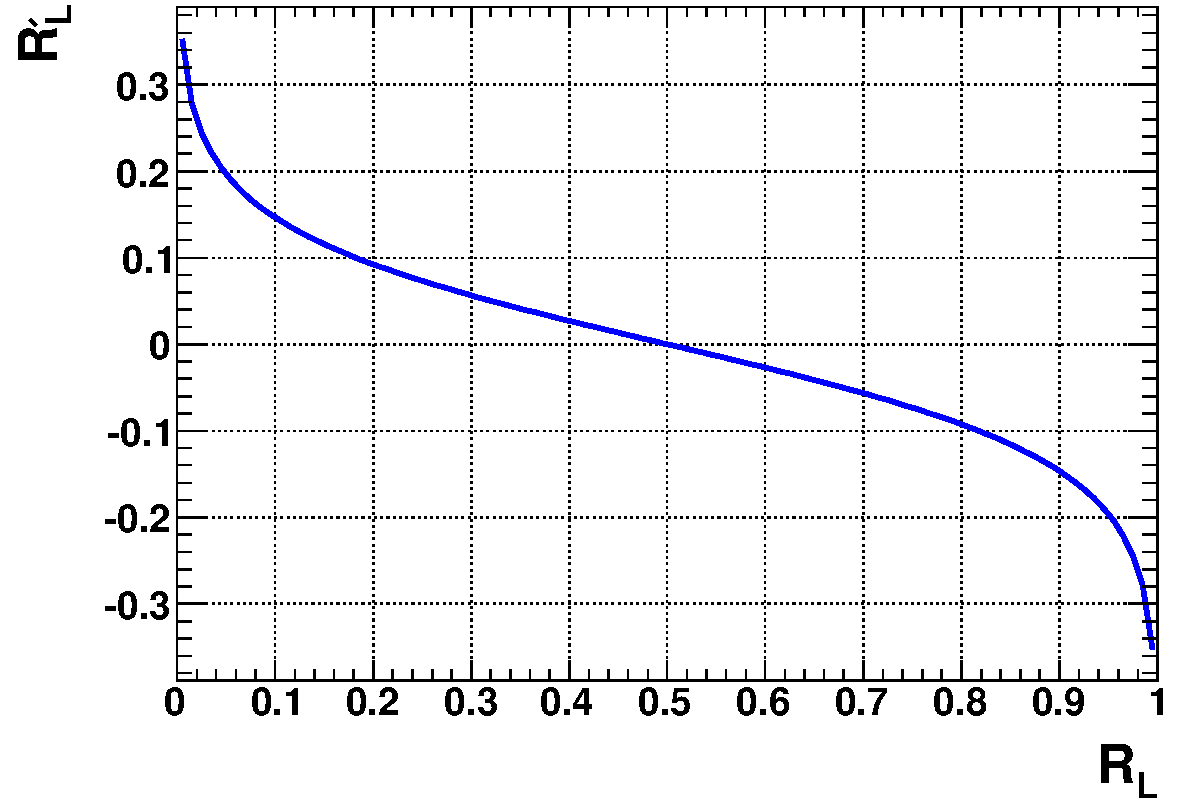
\includegraphics[width=0.53\textwidth]{plots/liktransform}
  \end{center}
  \vspace{-0.5cm}
  \caption[.]{Transformation~(\ref{eq:RLikTransformed}) of the likelihood output. }
\label{fig:liktransform}
\end{figure}

\subsubsection{Variable ranking}

The present likelihood implementation does not provide a ranking of 
the input variables.

\subsubsection{Performance}

Both the training and the application of the likelihood 
classifier are very fast operations that are suitable for large data sets. 

The performance of the classifier relies on the accuracy of the likelihood model.
Because high fidelity PDF estimates are mandatory, sufficient training statistics 
is required to populate the tails of the distributions.
The neglect of correlations between input variables in the model~(\ref{eq:Likelihood}), 
often leads to a diminution of the discrimination performance. While linear 
Gaussian correlations can be rotated away (see Sec.~\ref{sec:variableTransform}),
such an ideal situation is rarely given. Positive correlations lead to 
peaks at both $\RLik\to 0,1$. Correlations can be reduced by categorising 
the data samples and building an independent likelihood classifier for each 
event category. Such categories could be geometrical regions in the detector,
kinematic properties, etc. In spite of this, realistic applications with a 
large number of input variables are often plagued by irreducible correlations, 
so that projective likelihood approaches like the one discussed here are 
under-performing. This finding led to the development of the many 
alternative classifiers that exist in statistical theory today.

